\documentclass[]{report}
\usepackage[table,xcdraw]{xcolor}
\usepackage[Glenn]{fncychap}
\usepackage[T1]{fontenc}
\usepackage[francais]{babel}
\usepackage{wrapfig}
\usepackage{graphicx}
\usepackage[a4paper, width=175mm, top=15mm, bottom=25mm]{geometry}
\usepackage{parskip}
\usepackage{enumitem}
\usepackage{titlesec}
\usepackage{listings}
\usepackage{float}
\usepackage[final]{pdfpages}
\usepackage{tocbibind}
\usepackage{tocloft}
\usepackage{xpatch}
\usepackage{amsmath}
\usepackage{amsthm}
\usepackage{amsfonts}
\usepackage{graphics}
\usepackage{framed}
\usepackage{multirow}
\usepackage{graphicx}
\usepackage[utf8x]{inputenc}
\usepackage{mathtools}
\usepackage{amsmath}
\usepackage{tabularx}
\usepackage{tikz}
\usepackage{multirow}
\usepackage[noend]{algpseudocode}
\usepackage{tabularx}  % for tabularx


%\lstset{
%	literate=%
%	{à}{{\'a}}1
%	{í}{{\'i}}1
%	{é}{{\'e}}1
%	{è}{{\`e}}1
%	{ý}{{\'y}}1
%	{ú}{{\'u}}1
%	{ó}{{\'o}}1
%	{ě}{{\v{e}}}1
%	{š}{{\v{s}}}1
%	{č}{{\v{c}}}1
%	{ř}{{\v{r}}}1
%	{ž}{{\v{z}}}1
%	{ď}{{\v{d}}}1
%	{ť}{{\v{t}}}1
%	{ň}{{\v{n}}}1
%	{ů}{{\r{u}}}1
%	{Á}{{\'A}}1
%	{Í}{{\'I}}1
%	{É}{{\'E}}1
%	{Ý}{{\'Y}}1
%	{Ú}{{\'U}}1
%	{Ó}{{\'O}}1
%	{Ě}{{\v{E}}}1
%	{Š}{{\v{S}}}1
%	{Č}{{\v{C}}}1
%	{Ř}{{\v{R}}}1
%	{Ž}{{\v{Z}}}1
%	{Ď}{{\v{D}}}1
%	{Ť}{{\v{T}}}1
%	{Ň}{{\v{N}}}1
%	{Ů}{{\r{U}}}1
%}

\begin{document}


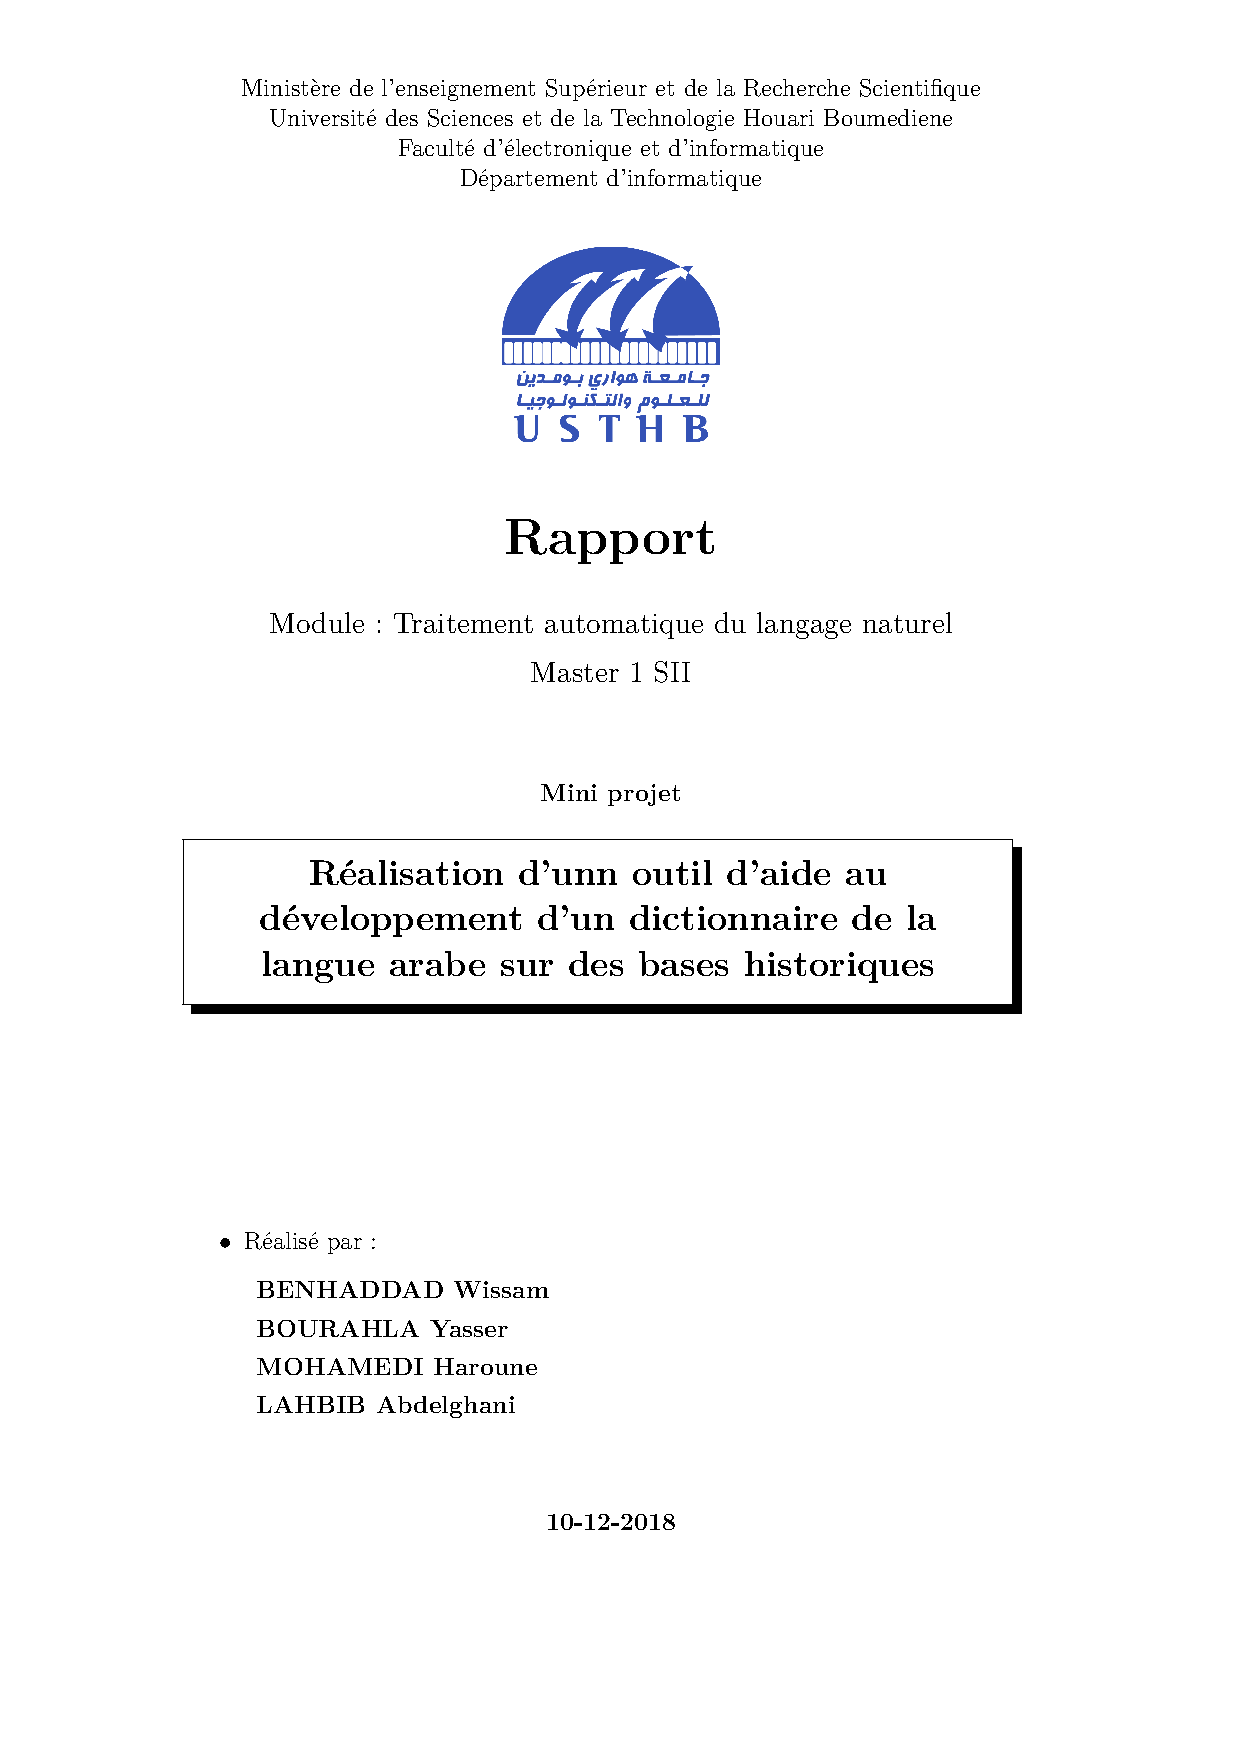
\includepdf[pages=1]{Page_garde.pdf} 

\tableofcontents

\listoffigures
	
\chapter{Motivations et problématique}
	\section{Introduction}
		\paragraph{}
		Depuis son apparition (au IIe siècle), la langue arabe n'a cessé d'évoluer, donnant naissance à de nouveaux mots, ou modifiant le sens de mots existants. Cette évolution a particulièrement enrichi le vocabulaire de la langue de l'islam, en conséquent et au fil du temps, plusieurs ouvrages destiné a recenser les différentes définitions et sens d'un mot ont vu le jour, chacun durant sa période. néanmoins,  il est primordial de garder une trace des différents changement qui ont eu lieu sur ces mots, et cela depuis leurs émergence. C'est avec cette idée en tête que les lexicographes des temps modernes en eu l'initiative d'entamer la construction de dictionnaires historiques afin de regrouper toutes les nuances des mots a travers les ages.
		\par
		La création d'un tel ouvrage n'est pas chose facile, en effet elle demande d'une part une grande connaissance sur les différentes périodes historiques de la langue, ainsi que sur la langue en elle même durant ces périodes. Chercher et regrouper des écrits, documents et ouvrages des différentes auteurs durant ces périodes est une tâche qui est en elle même très ardue, cela peut prendre plusieurs décennies pour créer une collection de documents asses représentative de chaque période. Analyser le contenue de tout ces documents est la phase qui dure le plus de temps, une vérification minutieuse de chaque information ajoutée au dictionnaire finale doit être faite, puis sujette à l'approbation de plusieurs experts du domaine.
		\par
		C'est avec l'avènement de l'informatique, de l'intelligence artificielle et plus récemment avec l'explosion du volume de données présent sur internet, que l'idée d'utiliser ces technologies pour faciliter et accélérer le processus de création d'un dictionnaire historique de la langue arabe à émergé. En effet la grande quantité et diversité de documents présente sur internet pourrait être exploité par un lexicographe pour ne pas s'attarder sur fastidieuse tâche de collecte des données, et cela en utilisant des techniques de traitement automatique du langage (TALN), de recherche d'information(RI) et d'intelligence artificielle.
		\par
		Ce besoin d'un outillage informatique est la principale motivation derrière ce mini-projet, avec suffisamment de données et une bonne conception, la réalisation d'un tel outillage pourrait faire gagner énormément de temps aux lexicographes du monde arabe.
		\par 
		Le but de projet étant maintenant établi, nous allons maintenant passer à la schématisation de ce rapport. Nous commencerons d'abord par de petites définitions pour se situer dans la suite du rapport, nous enchaînerons ensuite sur la conception du système pour expliquer le travail réalisé, viendra ensuite la présentation de notre application, enfin nous finirons par une conclusion générale comportant un bilan du projet, des critiques sur notre système ainsi que les perspectives envisagées.
	\section{Définitions}
		\subsection{DataSet et Corpus}
		\paragraph{}
		Un jeu de données (DataSet) est un ensemble de données traité et organisé dans un schéma spécifique aux besoins d'un système, un dataset peut être une base de données relationnelle, un ensemble de fichiers texte, une banque d'images/videos ...
		\par Dans notre cas nous nous intéresserons plus particulièrement à un type de dataset appelé Corpus, informellement un corpus est un dataset principalement utilisé dans le domaine du TALN, il est constitué d'un ensemble de fichier texte (annotés ou pas) qui représentent un domaine, une thématique, un(ou des) type(s) d'ouvrages ...
		\par Un corpus est un composant essentiel pour la l'application des techniques de TALN, la taille et la qualité d'un corpus est donc un facteur primordial pour assurer une bonne performance d'un système.
		\subsection{TALN}
			\paragraph{}
			Le Traitement Automatique du Langage Naturel (TALN) est un sous domaine de l'intelligence artificielle qui vise à analyser et à modéliser les composants du langage humain, que ce soit du point de vue syntaxique, sémantique ou pragmatique. l'aspect principal du TALN est le fait de permettre aux machine de traiter les séquence de texte non plus comme une simple suite de symboles, mais comme des entités informationnelles. Des connaissances sur la langue sont un prérequis essentiel pour le développement d'un système utilisant le TALN, ainsi que la disponibilité d'un grand ensemble de données pour faire de l'apprentissage automatique.
			\par 
			Le TALN est découpé en un ensemble de techniques et opérations à appliquer sur du texte, une multitude de domaine d'application existent pour l'utilisation de ces derniers. Dans ce projet nous nous intéresserons principalement aux techniques suivantes :  
			\subsubsection{Lemmatisation} 
				\paragraph{}
				La lemmatisation est un terme désignant l’analyse lexicale d’un texte dans le but de regrouper les mots d’une même famille. Les mots d’une même famille sont donc réduits en une unique entité appelée « \textbf{lemme} ».
				Ainsi la lemmatisation consiste à regrouper les différentes flexions d’un mot unique.\cite{lemme}
				
			\subsubsection{Segmentation}
				\paragraph{}
				La segmentation d'un texte est l'opération de découpage de ce dernier en composantes linguistiques plus petites(des phrases, des groupes nominaux, des mots ...), c'est un processus non-trivial car chaque langue dispose de règles spécifiques en ce qui concerne les marqueurs de fin de phrases.
			
			\subsubsection{Étiquetage morphosyntaxique (PoS-Tagging)}
				\paragraph{}
				il consiste à identifier pour chaque mot sa classe morphosyntaxique(Nom,Verbe,Nom pluriel, ...) à partir de son contexte dans un corpus ou texte ,ainsi que de connaissances lexicales de la langue.
			
		\subsection{Dictionnaire historique}
			\paragraph{}
			Informellement, un dictionnaire historique est un ouvrage qui rassemble, sous forme d'un liste d'entrées, un ensemble de mot d'une langue donnée avec leurs définitions et/ou des exemples d'utilisation selon des périodes historiques prédéfinies (en rapport avec la langue ou pas).
	\section{Conclusion}
	\paragraph{}
	Au terme de ce chapitre, nous avons une idée plus claire sur le travail qui doit être réaliser, nous allons donc attaquer l'aspect conceptualisation, il s'agira principalement de définir les composants de notre système.
	
\chapter{Conception du système}
	\section{Introduction}
	Comme mentionné précédemment, nous allons nous intéresser dans ce chapitre à la conception que nous avons réalisé, nous présenterons un schéma global du système, puis nous nous détaillerons le rôle de chaque composant, en donnant un exemple d'utilisation et/ou du flux de donnés qui entre/sort de ce dernier, nous parlerons ensuite du déploiement du système dans
	une plateforme serverless(dans le cloud), principalement car c'est un aspect important de l'expérience d'utilisation(UX).
	\section{Schéma global du système}
		\paragraph{}
		Notre système se compose essentiellement de deux parties(elles même subdivisées en plusieurs modules) : 
		\begin{itemize}
			\item \textbf{Récupération et pré-traitement des données } : principalement, c'est depuis des sites web que le système 
			cherche des données, puis il se charge d'organiser les fichiers téléchargés dans un espace de stockage.
			\item \textbf{Exploitation et mise à jour des données récupérées} : c'est la partie où les données qui sont maintenant
			structurées et organisées seront utilisées par l'application, qui dans notre cas se trouve être une application web hébergé dans le cloud.
		\end{itemize}
		\par 
		Le schémas suivant explicite un peu plus l'explication précédente : 
		
		\begin{figure}[H]
			\centering
			\includegraphics[width=0.75\linewidth]{ressources/schema.jpg}
			\caption{Schéma global du système}
			
		\end{figure}
		
	\section{Les modules du système}
		\paragraph{}
		Cette section se consacre à la description en détails des différentes modules du système, avec éventuellement des exemples d'utilisation de chacun.
		\subsection{Aspirateur de sites web}
			\paragraph{}
		\subsection{Organisateur de corpus}
		\subsection{Corpus reader}
		\subsection{Base de données}
		\subsection{Application (Front-end et Back-end)}		
	\section{Déploiement des modules dans le cloud}
		
	\section{Conclusion}


\chapter{Réalisation de l'application}
\section{Introduction}

\section{Environnement de travail et outils utilisés}
\subsection{Python}
\subsection{JavaScript}
\subsection{NLTK}
\subsection{VueJS}
\subsection{Django}
\subsection{PostgreSQL}
\subsection{Google Cloud Platform}

\section{Présentation de l'application}
	\subsection{Interface principale}
	Insert for each subsubsection an exemple of usage 
	\subsection{Corpus}
		\paragraph{}
		Upload new corpus into the server
	\subsection{Corpus Browser}
		\paragraph{}
		Explore the corporas
	\subsection{Add Entry}
		\paragraph{}
		Add new entries into the historical dico
	\subsection{Dicos}
		\paragraph{}
		All the words from the historical dico
	\subsection{Graphs}
		\paragraph{}
		Display different statistics for some words
\section{Fonctions supplémentaires}

\section{Conclusion}


\chapter{Conclusion générale}
\section{Objectifs atteints}
\section{Limites du système}
\section{Perspectives futures}		

%mode auto is simple: 
%3andek f corpus method trodlek "apparition generator"  tmedelha list of words, and restrictions over corpus like category, era, fileid .. ou howa idir lemma sentences ta3 corpus and each time issib a word fhadouk lemmas irodlek the word m3a (fileid, sentence position fel file, word position fel sentence, a chunk of the sentence[optional]
\bibliographystyle{ieeetr}
\bibliography{ref}

\end{document}